\section{Experiments and results}
\label{sec:experiments}

We evaluate JaxARC along three axes. First, we measure whether the environment is practical enough to support repeated ARC adaptation studies at the scale required for the benchmark. Second, we keep one archived MiniARC ablation as a narrow diagnostic of interface learnability under privileged observations. Third, and most importantly, we evaluate whether task-specific PPO adaptation improves hidden-query performance under the canonical support/query protocol.

\subsection{Practicality benchmark: throughput against ARCLE}

\paragraph{Experimental design.}
We compare archived H100 throughput benchmarks for JaxARC and ARCLE on a single fixed ARC task. Each benchmark call executes 100 environment steps and is repeated 10 times per batch size. For JaxARC, we report steady-state throughput after the one-time JIT compilation step. ARCLE is measured in its synchronous and asynchronous Python implementations, both without any compile phase. The comparison is therefore a simulator-throughput benchmark on matched environment calls, not a fully matched end-to-end adaptation run.

\begin{figure}[t]
\centering
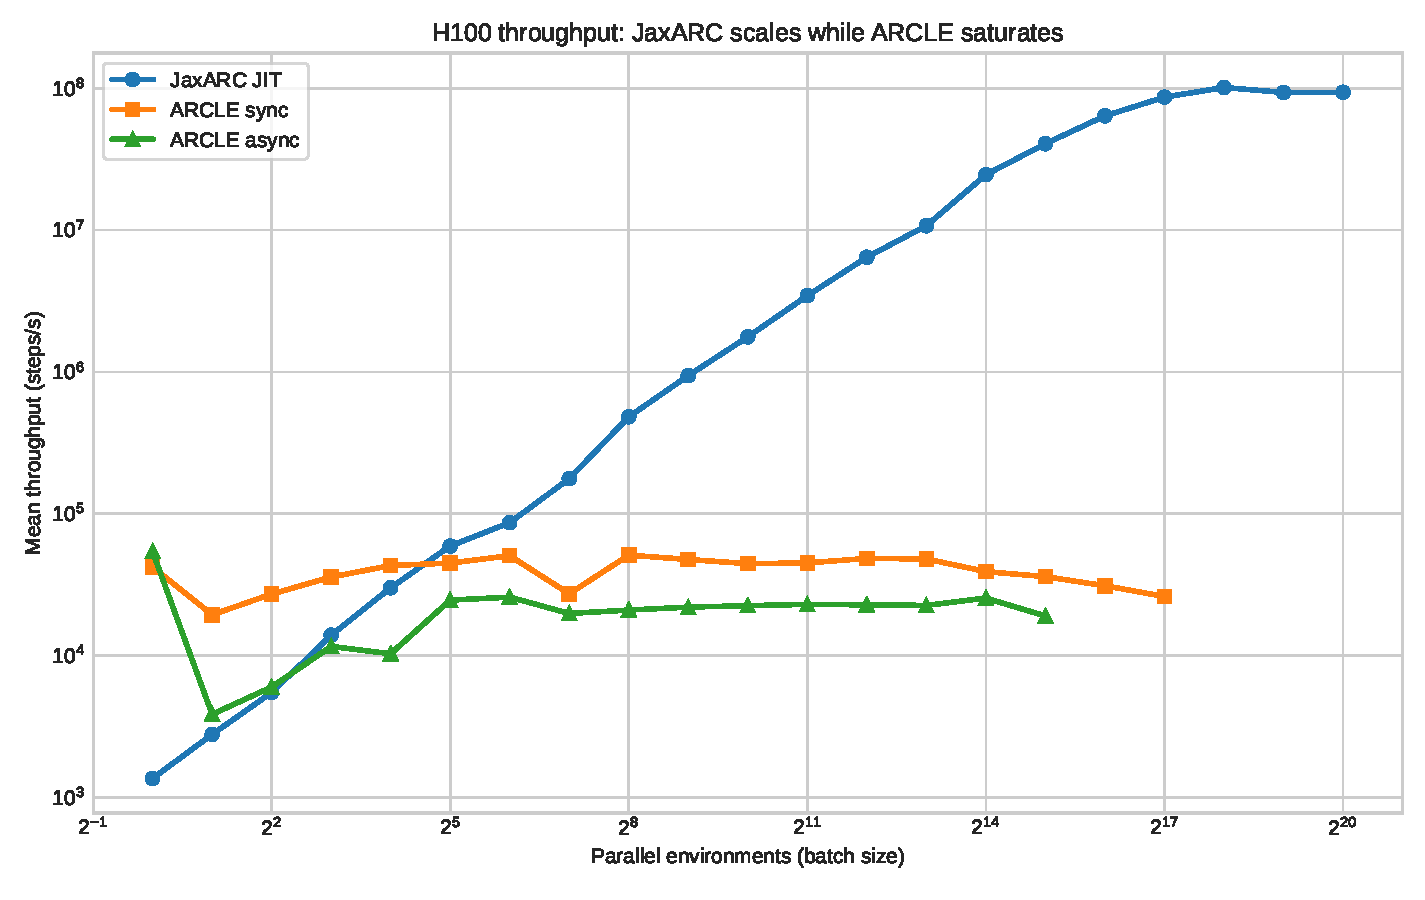
\includegraphics[width=0.9\linewidth]{Figures/h100_throughput_vs_batch.pdf}
\caption{Throughput on the archived H100 practicality benchmark. Each point reports mean environment steps per second for 100-step benchmark calls, averaged over 10 repeats on a fixed ARC task. JaxARC is measured after one-time compilation, while ARCLE is measured in its synchronous and asynchronous Python modes.}
\label{fig:h100_throughput_vs_batch}
\end{figure}

\paragraph{Results.}
Figure~\ref{fig:h100_throughput_vs_batch} shows a large throughput gap in favor of JaxARC. Peak post-compilation JaxARC throughput reaches 101{,}311{,}134 steps/s at batch 262{,}144. The archived ARCLE baselines peak at 51{,}035 steps/s for the synchronous implementation at batch 256 and 54{,}082 steps/s for the asynchronous implementation at batch 1 \citep{leeARCLEAbstractionReasonin2024}. On matched batch sizes, the best archived speedups are 3323.2$\times$ over ARCLE sync and 2138.9$\times$ over ARCLE async. We treat this result as a practicality claim rather than a stand-alone scientific result: the main point is that JaxARC makes large budget ladders, ablations, and repeated task-level evaluation cheap enough to run as a benchmark rather than as isolated demonstrations.

\subsection{PPO diagnostic: observation wrappers on MiniARC}

\paragraph{Experimental design.}
We retain one archived MiniARC pilot because it answers a narrow but useful question: under a simplified setting, does PPO learn the JaxARC interface more easily when the observation exposes more information? The pilot uses Stoix feedforward PPO with the shallow CNN baseline (\texttt{arc\_shallow\_cnn}), a 500M-step training budget, point actions, a 150-step episode limit, and the balanced reward setting used in the early JaxARC baselines. The sweep covers seven observation configurations: working grid only; working grid plus answer; working grid plus input; working grid plus contextual support examples; and the three corresponding combinations.

\begin{figure}[t]
\centering
\begin{minipage}[t]{0.49\linewidth}
    \centering
    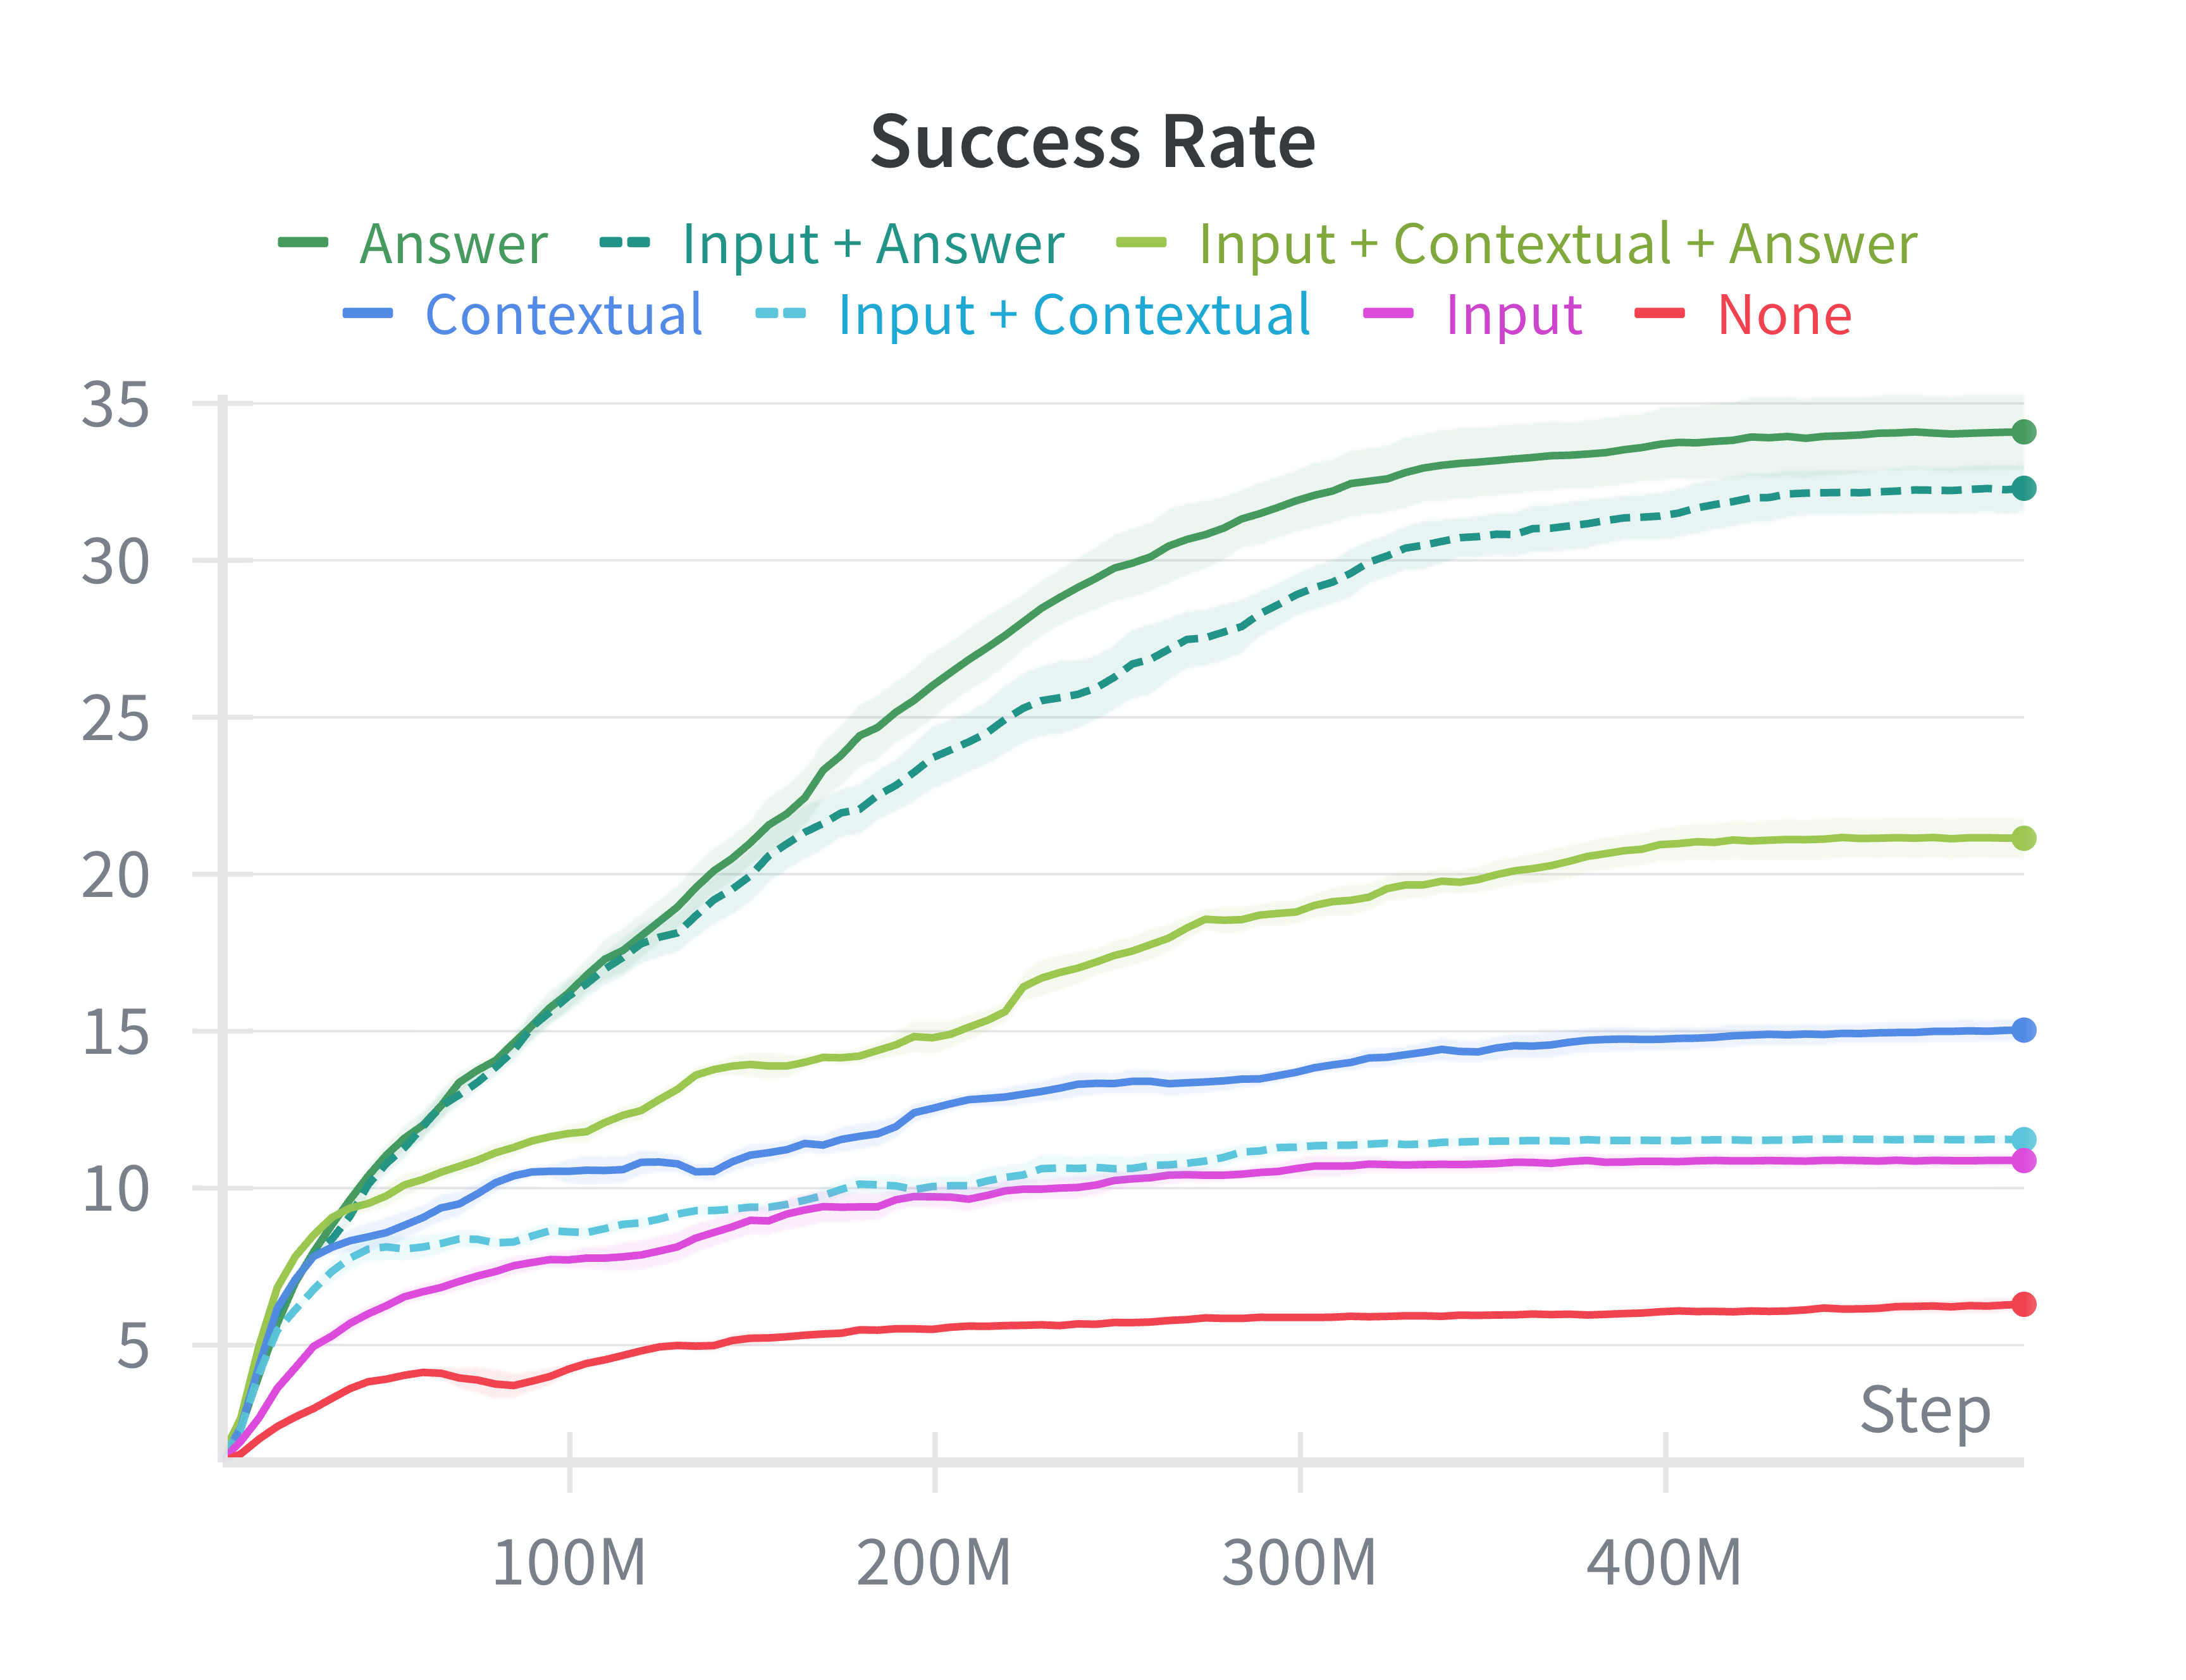
\includegraphics[width=\linewidth]{Figures/mini_success_rate_obs_config.png}
\end{minipage}\hfill
\begin{minipage}[t]{0.49\linewidth}
    \centering
    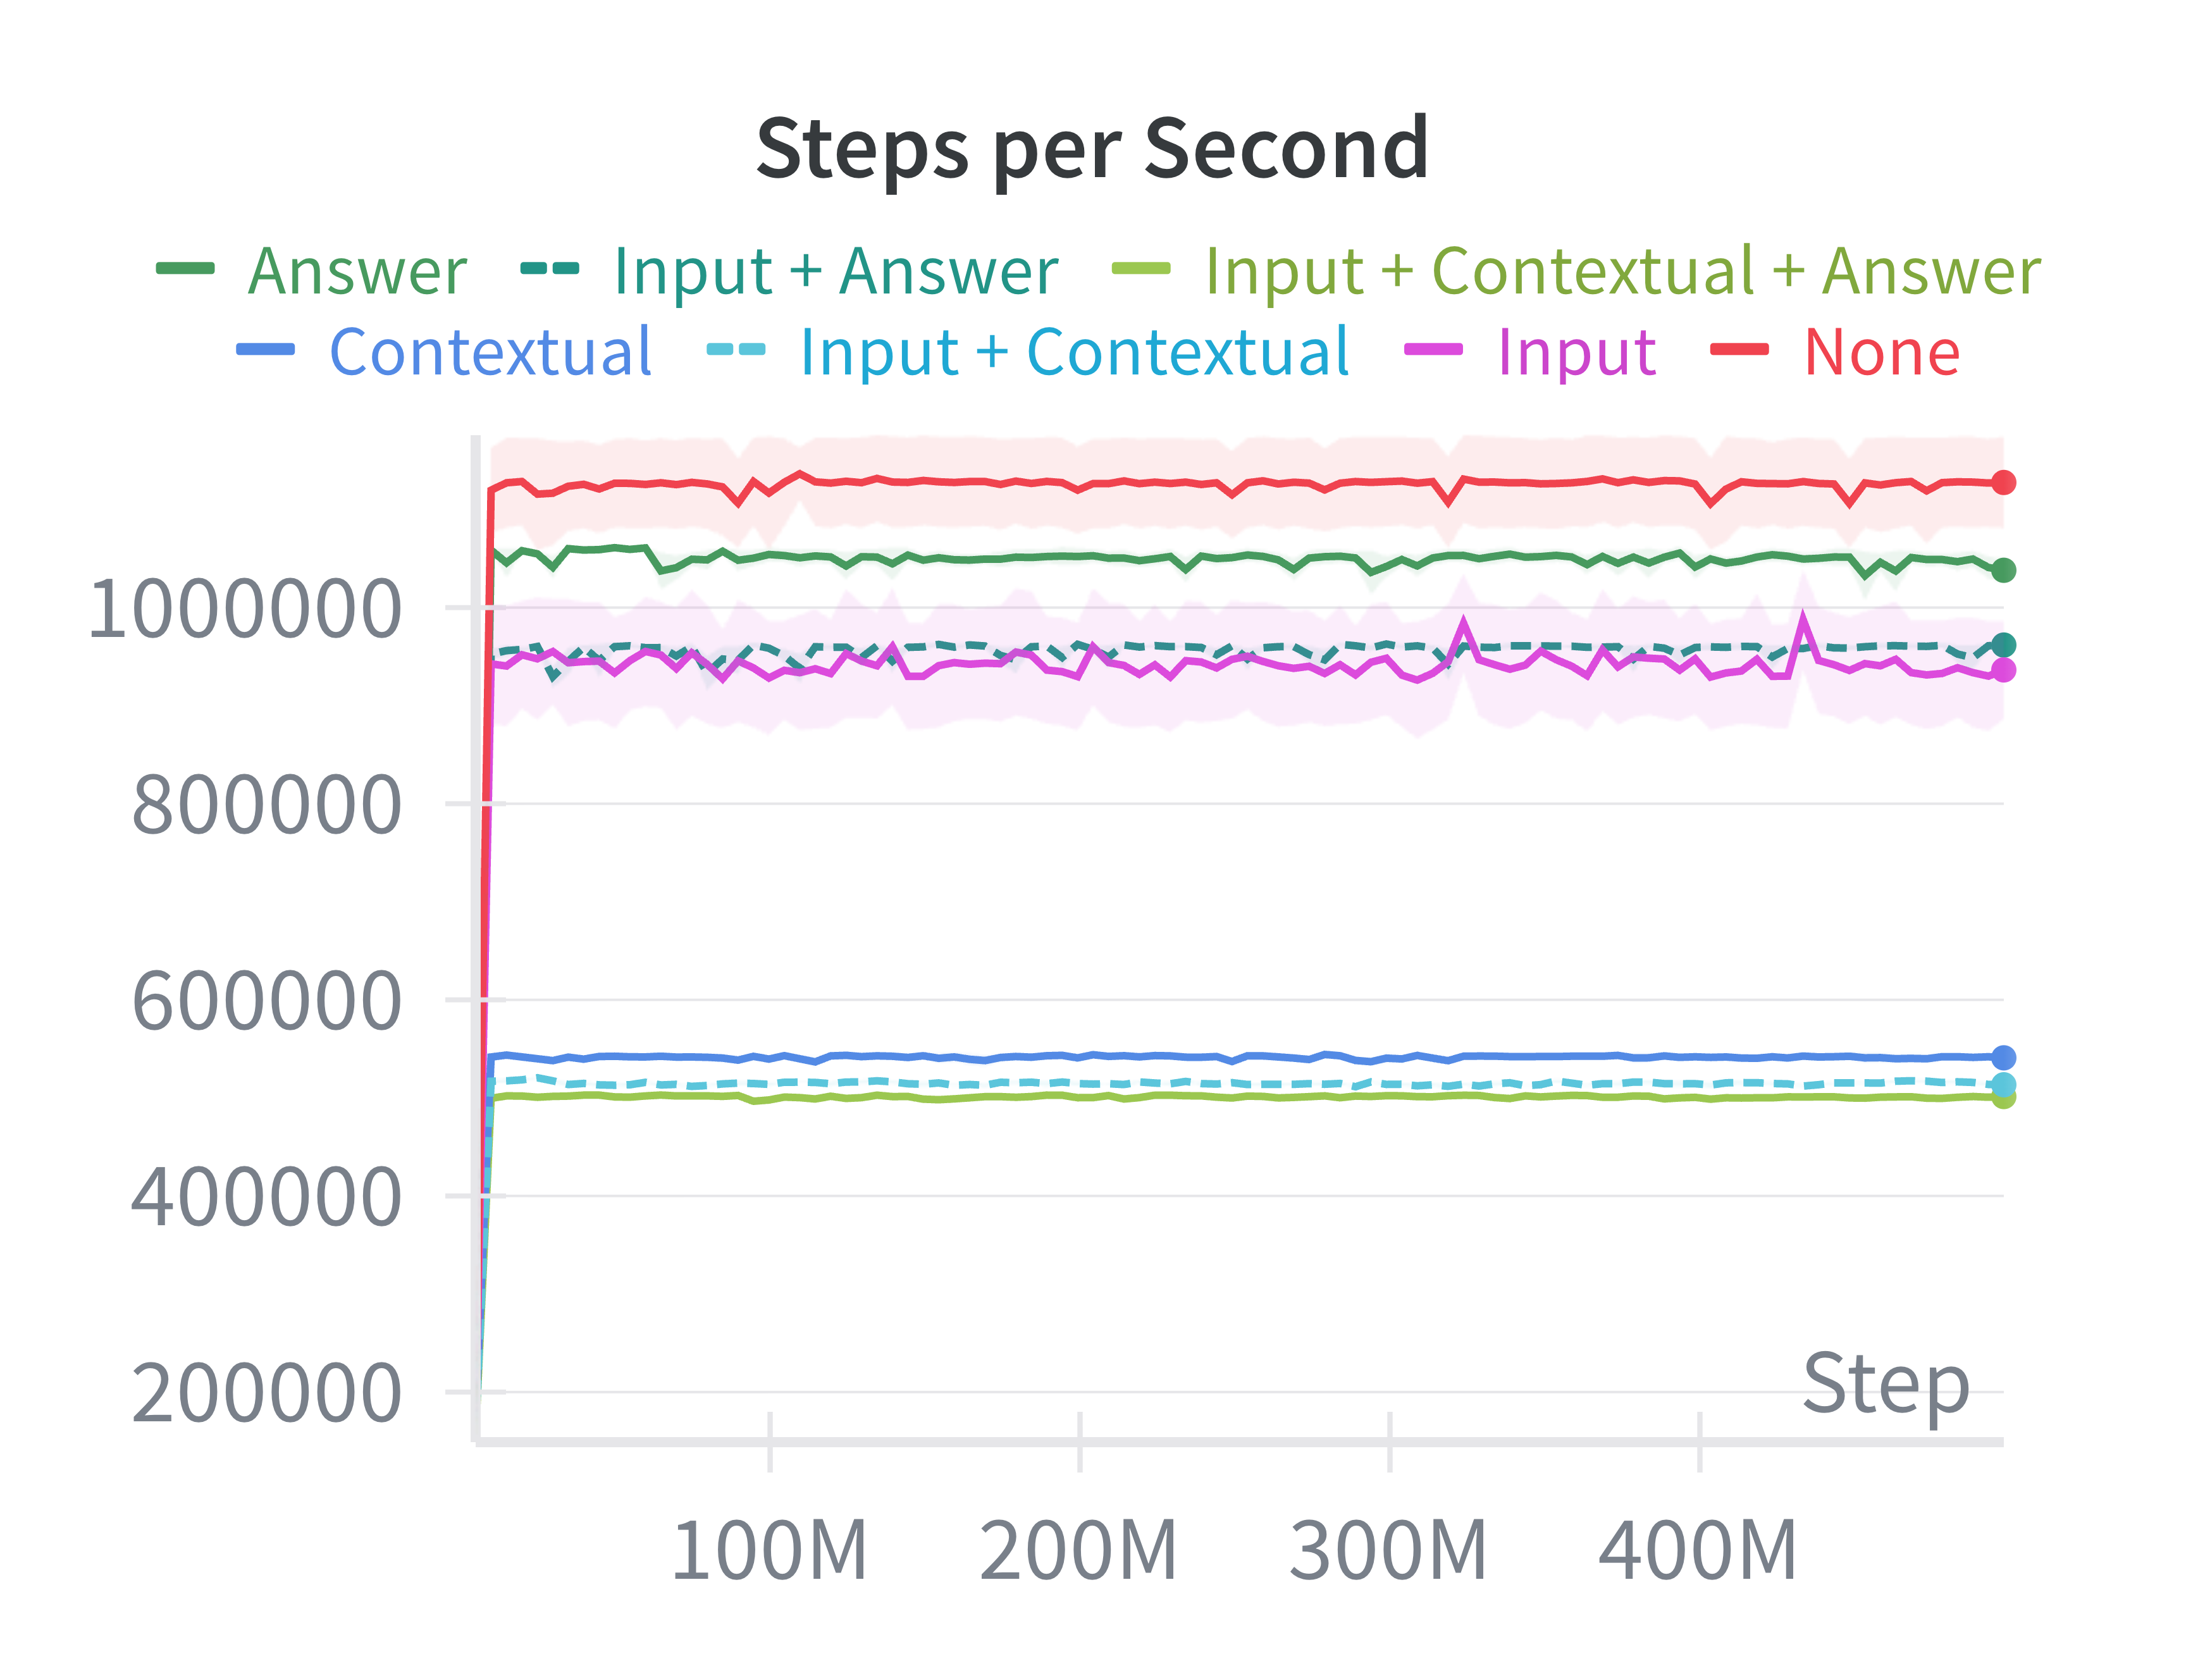
\includegraphics[width=\linewidth]{Figures/mini_sps_obs_config.png}
\end{minipage}
\caption{Archived MiniARC observation-wrapper diagnostic reused from the earlier manuscript draft. Left: success-rate curves for seven observation configurations. Right: training throughput. This figure is included as a narrow diagnostic about interface learnability, not as part of the canonical support/query benchmark package.}
\label{fig:ppo_obs_diagnostic}
\end{figure}

\paragraph{Results.}
Figure~\ref{fig:ppo_obs_diagnostic} suggests two stable qualitative patterns. First, answer-visible configurations are much easier than configurations that hide the answer. In this privileged setting, PPO can learn action sequences more readily when the desired target grid is present in the observation. Second, wider observations do not help monotonically. Adding input and contextual channels does not consistently outperform the simpler answer-visible conditions, and the throughput panel shows the expected cost of those extra channels. We therefore use this pilot only as a sanity check that privileged target access can make the control problem easier for a shallow PPO baseline, similar in spirit to simplified ARCLE diagnostics \citep{leeARCLEAbstractionReasonin2024}. It is not evidence of hidden-query transfer under the canonical benchmark.

\subsection{Canonical task-specific adaptation benchmark}

\paragraph{Experimental design.}
The main benchmark allocates a fixed per-task interaction budget on support pairs and then evaluates the adapted policy on hidden query pairs whose targets remain masked from the agent-visible state. During query evaluation, the environment scores the hidden target internally, but the policy receives no target-revealing similarity reward. The canonical ARC-AGI-1 series uses 27 entry-level ARC-AGI-1 training tasks \citep{cholletMeasureIntelligence2019}. We report a no-adaptation anchor together with three PPO variants: feedforward PPO, pretrained feedforward PPO, and recurrent PPO. All completed AGI1 canonical runs use point actions, the input/answer/context observation stack, a 150-step episode limit, balanced reward shaping during support adaptation, and the restricted operation set $\{0,\ldots,9,33,34\}$. The budget ladder is 0, 10k, 50k, and 100k environment timesteps per task. To test whether the same pattern appears beyond ARC-AGI-1, we also include completed feedforward PPO series on MiniARC and ConceptARC \citep{kimPlaygroundsAbstractionReasoning2022,moskvichevConceptARCBenchmarkEvaluating2023}.

We report five task-aggregated metrics. \emph{Support similarity} is the mean fraction of target cells matched on support episodes. \emph{Query exact success rate} requires a submitted answer that exactly matches the hidden target. \emph{Query final-grid match rate} measures exact agreement between the terminal grid and the hidden target regardless of whether the policy submitted. \emph{Query similarity} is the mean target-cell match fraction on the terminal query grid. \emph{Submitted-query rate} records how often the policy chooses to submit on hidden queries.

\begin{figure}[t]
\centering
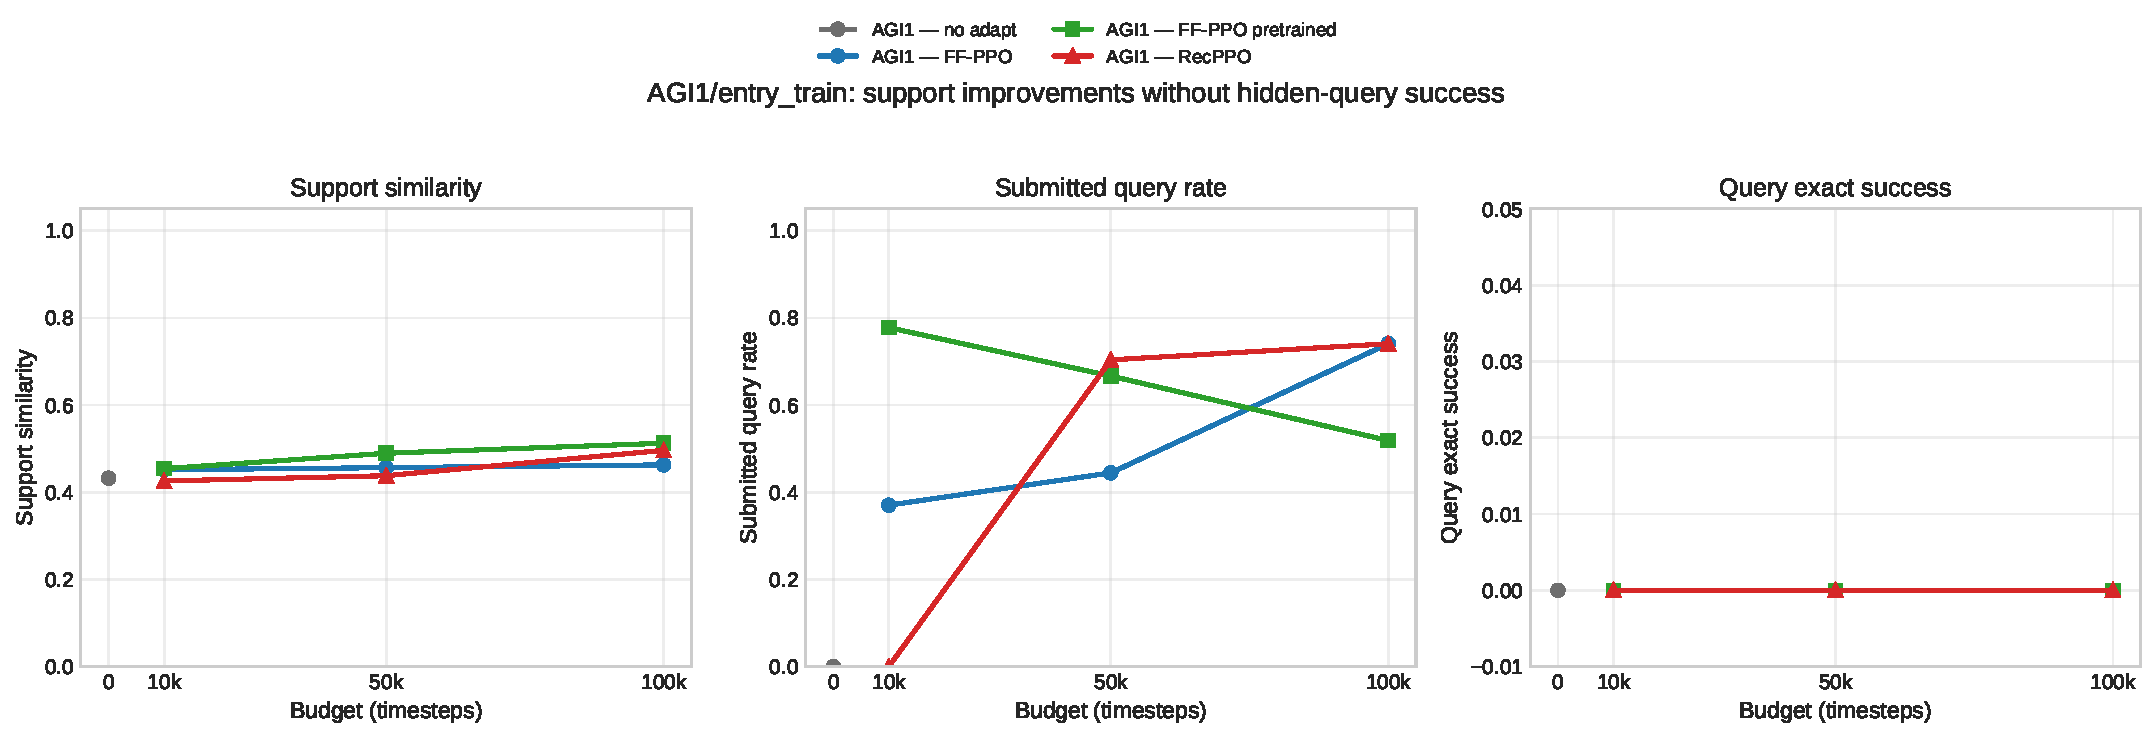
\includegraphics[width=0.92\linewidth]{Figures/agi1_budgeted_profile.pdf}
\caption{Canonical ARC-AGI-1 task-specific adaptation benchmark. At larger budgets, the PPO variants improve support similarity and can change submission behavior on hidden queries, but hidden-query exact success remains zero throughout the completed canonical series.}
\label{fig:agi1_budgeted_profile}
\end{figure}

\paragraph{Results.}
Figure~\ref{fig:agi1_budgeted_profile} captures the main empirical result of the paper. On ARC-AGI-1, the no-adaptation anchor starts at mean support similarity 0.432. At the strongest completed budget, feedforward PPO reaches 0.463, pretrained feedforward PPO reaches 0.513, and recurrent PPO reaches 0.496. These are real support-side changes. They do not, however, produce hidden-query correctness: query exact success rate, query final-grid match rate, and query similarity are all 0.000 for every completed ARC-AGI-1 canonical series in the packaged benchmark summary.

The same separation appears away from ARC-AGI-1. At 100k, MiniARC feedforward PPO reaches support similarity 0.708 over 68 completed tasks, while query exact success remains 0.000. On ConceptARC, feedforward PPO reaches support similarity 0.797 over 50 completed tasks, again with query exact success 0.000. Submission behavior changes without becoming correctness. On ARC-AGI-1 at 100k, feedforward PPO and recurrent PPO each submit on 0.741 of hidden-query episodes, while pretrained feedforward PPO submits on 0.519, yet all three remain at zero query exact success.

The gap is also visible at the task level. At 100k, 5/27 ARC-AGI-1 feedforward PPO tasks and 6/27 ARC-AGI-1 pretrained PPO tasks reach support similarity at least 0.8 while still recording zero query exact success. On ConceptARC, the same pattern appears on 36/50 tasks, including 5/50 tasks that reach support similarity 1.0 and still have zero hidden-query exact success. These counts rule out the trivial reading that the benchmark is only measuring uniformly weak policies. The policies often do fit the visible support pairs, and they sometimes become more willing to submit on hidden queries. What does not emerge in the completed canonical series is transfer from support-side fitting to hidden-query correctness.
